% !TeX root = ../../../main.tex
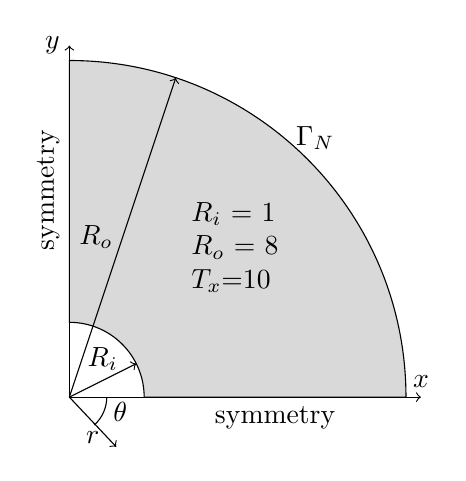
\begin{tikzpicture}[scale=0.95]%
%
\def\drawcenterarc[#1](#2)(#3:#4:#5)% Syntax: [draw options] (center) (initial angle:final angle:radius)
{ \draw[#1] ($(#2)+({#5*cos(#3)},{#5*sin(#3)})$) arc (#3:#4:#5); };
\def\centerarc[#1](#2)(#3:#4:#5)% Syntax: [draw options] (center) (initial angle:final angle:radius)
{ ($(#2)+({#5*cos(#3)},{#5*sin(#3)})$) arc (#3:#4:#5) };
%
\def\innerRadius{1};
\def\outerRadius{4.5};
\draw [ fill=black!15 ] 
(\innerRadius,0) -- (\outerRadius,0) 
node[midway, below]{symmetry}  
arc (0:90:\outerRadius) 
%\centerarc[](0,0)(0:90:\outerRadius)
node[midway, right, above, xshift=0.1cm]{$ \Gamma_N $}
 -- (0,\innerRadius) 
node[midway, left, rotate=90, xshift=0.9cm,yshift=0.27cm]{symmetry} 
 arc (90:0:\innerRadius);%
 %\centerarc[](0,0)(0:90:\innerRadius);
 
%
\draw [ -> ] (0,0) -- (\innerRadius*0.894427191, \innerRadius*0.447213595) node[midway, above]{$ R_i $};
\draw [ -> ] (0,0) -- (\outerRadius*0.316227766, \outerRadius*0.948683298) node[midway, left]{$ R_o $};
%
%\draw [ -> ] (0,0) -- (\innerRadius*0.7*0.8, -\innerRadius*0.7*0.6) node[midway, above]{$ r $};
%\draw [ ] (\innerRadius*0.5,0) arc (36.869897646:0:\innerRadius*0.5) node[midway, right]{$ \theta $} ;
%
\draw [ -> ] (0,0) -- (\innerRadius*0.7*0.894427191, -\innerRadius*0.7*0.948683298) node[midway, below]{$ r $};
\draw [ ] (\innerRadius*0.5,0) arc (0:-48:\innerRadius*0.5) node[midway, right]{$ \theta $} ;
%
\draw [ -> ] (0,0) -- (\outerRadius + \innerRadius/5,0) node[ above]{$x$};
\draw [ -> ] (0,0) -- (0,\outerRadius + \innerRadius/5) node[ left]{$y$};
%
\draw[] (1.5,2) node[text width=3cm,right] {$R_i$ = 1\\$R_o$ = 8\\$T_x$=10};
%
%
\end{tikzpicture}%